\documentclass[12pt]{article}
\usepackage[utf8]{inputenc}
\usepackage{graphicx}
\usepackage{subcaption}
\usepackage{amsmath}
\usepackage{fancyhdr}
\usepackage{geometry}
\usepackage{float}
\usepackage{listings}
\usepackage{xcolor}
\usepackage{array}
\usepackage{caption}
\usepackage{booktabs}
\usepackage[english]{babel}
\usepackage{hyperref}

\lstset{
    basicstyle=\ttfamily\footnotesize,
    backgroundcolor=\color{gray!10},
    keywordstyle=\color{blue},
    commentstyle=\color{green!50!black},
    stringstyle=\color{red},
    numbers=left,
    numberstyle=\tiny\color{gray},
    stepnumber=1,
    numbersep=10pt,
    showstringspaces=false,
    frame=single,
    tabsize=4,
    breaklines=true,
    breakatwhitespace=false,
    language=Java
}

\linespread{1.25}
\setlength{\parindent}{0.8cm}
\setlength{\parskip}{0em}
\renewcommand{\headrulewidth}{0pt}
\geometry{a4paper, portrait, margin=1in}
\setlength{\headheight}{14.49998pt}
\graphicspath{{Lab2/charts/}}

\begin{document}

% ─── TITLE PAGE ───────────────────────────────────────────────────────────────
\begin{titlepage}
  \begin{center}
    \textbf{\large Ministry of Education of Republic of Moldova}\\[0.1cm]
    \textbf{\large Technical University of Moldova}\\[0.1cm]
    \textbf{\large Faculty of Computers, Informatics and Microelectronics}\\[1.2cm]

    \vspace{40mm}

    \textsc{\Large Laboratory Work 2:}\\[0.2cm]
    \textsc{\Large Study and Empirical Analysis of Sorting Algorithms}\\[0.4cm]

    \vspace{65mm}

    \begin{minipage}[t]{0.4\textwidth}
      \begin{flushleft}\large
        \emph{Author:}\\
        st. gr. FAF-242\\[0.4cm]
        \emph{Verified:}\\
        asist. univ.
      \end{flushleft}
    \end{minipage}
    ~
    \begin{minipage}[t]{0.4\textwidth}
      \begin{flushright}\large
        \emph{}\\
        Tacu Igor\\[0.4cm]
        \emph{}\\
        Fiștic Cristofor
      \end{flushright}
    \end{minipage}\\[2cm]

    \vspace{5mm}
    \large Chișinău -- 2025

    \vfill
  \end{center}
\end{titlepage}

% ─── TABLE OF CONTENTS ────────────────────────────────────────────────────────
\clearpage
\thispagestyle{empty}
\tableofcontents

\clearpage
\setcounter{page}{2}
\pagestyle{fancy}
\fancyhf{}
\rhead{\thepage}

% ─── 1. OBJECTIVE & TASKS ─────────────────────────────────────────────────────
\section*{OBJECTIVE}
\addcontentsline{toc}{section}{OBJECTIVE}

Study and empirically analyze the most common comparison-based sorting algorithms, measuring
their execution time across multiple input types and sizes, and identify each algorithm's
strengths and limitations in practice.

\subsection*{Tasks}
\addcontentsline{toc}{subsection}{Tasks}

\begin{enumerate}
  \item Implement four sorting algorithms: QuickSort, MergeSort, HeapSort, and BubbleSort.
  \item Design the input format (sizes and types) for the empirical analysis.
  \item Select execution time as the comparison metric.
  \item Run each algorithm on three input types: random, sorted, and reverse-sorted.
  \item Generate graphical representations of the results.
  \item Test algorithms on edge-case inputs (empty arrays, nulls, NaN, complex numbers).
  \item Deduce conclusions from the obtained data.
\end{enumerate}

% ─── 2. THEORETICAL BACKGROUND ───────────────────────────────────────────────
\section*{THEORETICAL BACKGROUND}
\addcontentsline{toc}{section}{THEORETICAL BACKGROUND}

\subsection*{Empirical Analysis}
\addcontentsline{toc}{subsection}{Empirical Analysis}

\hspace{0.8cm} Empirical analysis is an experimental approach to measuring algorithm efficiency.
Rather than deriving complexity through mathematical reasoning alone, the algorithm is implemented
and executed on controlled input datasets, and the observed metrics (here: wall-clock execution time)
are recorded and plotted. This approach is especially useful when:

\begin{itemize}
  \item the mathematical analysis is complex or unavailable;
  \item comparing practical performance of algorithms with identical asymptotic complexity;
  \item assessing the impact of hardware and implementation details on real runtimes.
\end{itemize}

Each algorithm was run \textbf{5 times} per input size, and the \textbf{average} time (in milliseconds) was
recorded to smooth out noise from OS scheduling and JVM warm-up effects.

\subsection*{Sorting Algorithms Overview}
\addcontentsline{toc}{subsection}{Sorting Algorithms Overview}

\hspace{0.8cm} The four algorithms selected span a range of asymptotic complexities and practical
behaviors, making them a representative sample for comparison:

\begin{center}
\renewcommand{\arraystretch}{1.4}
\begin{tabular}{lcccc}
\toprule
\textbf{Algorithm} & \textbf{Best Case} & \textbf{Average Case} & \textbf{Worst Case} & \textbf{Space} \\
\midrule
QuickSort   & $O(n \log n)$ & $O(n \log n)$ & $O(n^2)$      & $O(\log n)$ \\
MergeSort   & $O(n \log n)$ & $O(n \log n)$ & $O(n \log n)$ & $O(n)$      \\
HeapSort    & $O(n \log n)$ & $O(n \log n)$ & $O(n \log n)$ & $O(1)$      \\
BubbleSort  & $O(n)$        & $O(n^2)$      & $O(n^2)$      & $O(1)$      \\
\bottomrule
\end{tabular}
\captionof{table}{Theoretical time and space complexity of the four sorting algorithms.}
\end{center}

% ─── 3. INPUT FORMAT ──────────────────────────────────────────────────────────
\section*{INPUT FORMAT}
\addcontentsline{toc}{section}{INPUT FORMAT}

\hspace{0.8cm} Each algorithm was tested against two sets of input sizes:

\begin{itemize}
  \item \textbf{Full set} (all 4 algorithms, including BubbleSort):\\
        $n \in \{250,\ 500,\ 750,\ 1000,\ 1500,\ 2000,\ 3000,\ 4000,\ 5000,\ 7500,\ 10000,\ 15000,\ 20000\}$

  \item \textbf{Large set} (QuickSort, MergeSort, HeapSort only):\\
        $n \in \{500,\ 1000,\ 2000,\ 5000,\ 10000,\ 20000,\ 40000,\ 60000,\ 80000,\ 100000\}$
\end{itemize}

For every size $n$, three input arrays were generated:

\begin{enumerate}
  \item \textbf{Random} -- values drawn uniformly from $[0, 100000)$ using a fixed seed.
  \item \textbf{Sorted} -- array $[0, 1, 2, \ldots, n-1]$; represents the best case for some algorithms.
  \item \textbf{Reverse-sorted} -- array $[n, n-1, \ldots, 1]$; represents a common worst case.
\end{enumerate}

% ─── 4. IMPLEMENTATION ────────────────────────────────────────────────────────
\section*{IMPLEMENTATION}
\addcontentsline{toc}{section}{IMPLEMENTATION}

\hspace{0.8cm} All four algorithms were implemented in Java using a Maven project structure.
Each class provides two overloads: a primitive \texttt{int[]} version for the empirical benchmarks,
and a generic \texttt{T[] + Comparator<T>} version used in edge-case testing.
The timing harness runs the sort 5 times on a fresh copy of the input and returns the average.

\subsection*{QuickSort}
\addcontentsline{toc}{subsection}{QuickSort}

\hspace{0.8cm} QuickSort partitions the array around a pivot and recursively sorts each partition.
The naive last-element pivot causes $O(n^2)$ performance on sorted inputs; to avoid this,
a \textbf{median-of-three} pivot selection strategy was implemented: the median of
\texttt{arr[low]}, \texttt{arr[mid]}, and \texttt{arr[high]} is chosen and placed at
\texttt{arr[high]} before partitioning.

\begin{lstlisting}[caption={QuickSort -- median-of-three pivot and partition}, label={lst:qs}]
static int medianOfThree(int[] arr, int low, int high) {
    int mid = low + (high - low) / 2;
    if (arr[low] > arr[mid])  swap(arr, low, mid);
    if (arr[low] > arr[high]) swap(arr, low, high);
    if (arr[mid] > arr[high]) swap(arr, mid, high);
    swap(arr, mid, high); // pivot -> arr[high]
    return arr[high];
}

static int partition(int[] arr, int low, int high) {
    if (high - low >= 2) medianOfThree(arr, low, high);
    int pivot = arr[high], i = low - 1;
    for (int j = low; j < high; j++)
        if (arr[j] < pivot) swap(arr, ++i, j);
    swap(arr, i + 1, high);
    return i + 1;
}

static void quickSort(int[] arr, int low, int high) {
    if (low < high) {
        int pi = partition(arr, low, high);
        quickSort(arr, low, pi - 1);
        quickSort(arr, pi + 1, high);
    }
}
\end{lstlisting}

\subsection*{MergeSort}
\addcontentsline{toc}{subsection}{MergeSort}

\hspace{0.8cm} MergeSort divides the array in half, recursively sorts both halves, and merges them.
Its $O(n \log n)$ worst-case guarantee makes it stable and predictable across all input types.
A common bug -- omitting \texttt{k++} in the final merge loop -- was present in the skeleton
and has been fixed.

\begin{lstlisting}[caption={MergeSort -- merge step}, label={lst:ms}]
static void merge(int[] arr, int l, int m, int r) {
    int[] L = Arrays.copyOfRange(arr, l, m + 1);
    int[] R = Arrays.copyOfRange(arr, m + 1, r + 1);
    int i = 0, j = 0, k = l;
    while (i < L.length && j < R.length)
        arr[k++] = (L[i] <= R[j]) ? L[i++] : R[j++];
    while (i < L.length) arr[k++] = L[i++];
    while (j < R.length) arr[k++] = R[j++]; // bug fix: k++ was missing
}

static void mergeSort(int[] arr, int l, int r) {
    if (l < r) {
        int m = l + (r - l) / 2;
        mergeSort(arr, l, m);
        mergeSort(arr, m + 1, r);
        merge(arr, l, m, r);
    }
}
\end{lstlisting}

\subsection*{HeapSort}
\addcontentsline{toc}{subsection}{HeapSort}

\hspace{0.8cm} HeapSort builds a max-heap from the input array, then repeatedly extracts the maximum
element to produce a sorted sequence. It achieves $O(n \log n)$ in all cases and operates in-place.

\begin{lstlisting}[caption={HeapSort -- heapify and sort}, label={lst:hs}]
static void heapify(int[] arr, int n, int i) {
    int largest = i, l = 2*i+1, r = 2*i+2;
    if (l < n && arr[l] > arr[largest]) largest = l;
    if (r < n && arr[r] > arr[largest]) largest = r;
    if (largest != i) {
        int tmp = arr[i]; arr[i] = arr[largest]; arr[largest] = tmp;
        heapify(arr, n, largest);
    }
}

static void heapSort(int[] arr) {
    int n = arr.length;
    for (int i = n/2 - 1; i >= 0; i--) heapify(arr, n, i);
    for (int i = n - 1; i > 0; i--) {
        int tmp = arr[0]; arr[0] = arr[i]; arr[i] = tmp;
        heapify(arr, i, 0);
    }
}
\end{lstlisting}

\subsection*{BubbleSort}
\addcontentsline{toc}{subsection}{BubbleSort}

\hspace{0.8cm} BubbleSort repeatedly passes through the array, swapping adjacent elements that are out
of order. An early-exit flag (\texttt{swapped}) is used so that the algorithm terminates in $O(n)$ when
the input is already sorted -- which is reflected clearly in the empirical results.

\begin{lstlisting}[caption={BubbleSort -- with early-exit optimization}, label={lst:bs}]
static void bubbleSort(int[] arr, int n) {
    for (int i = 0; i < n - 1; i++) {
        boolean swapped = false;
        for (int j = 0; j < n - i - 1; j++) {
            if (arr[j] > arr[j + 1]) {
                int tmp = arr[j]; arr[j] = arr[j+1]; arr[j+1] = tmp;
                swapped = true;
            }
        }
        if (!swapped) break; // already sorted
    }
}
\end{lstlisting}

% ─── 5. RESULTS & ANALYSIS ────────────────────────────────────────────────────
\section*{RESULTS AND ANALYSIS}
\addcontentsline{toc}{section}{RESULTS AND ANALYSIS}

\subsection*{All Algorithms -- Random Input}
\addcontentsline{toc}{subsection}{All Algorithms -- Random Input}

\begin{figure}[H]
  \centering
  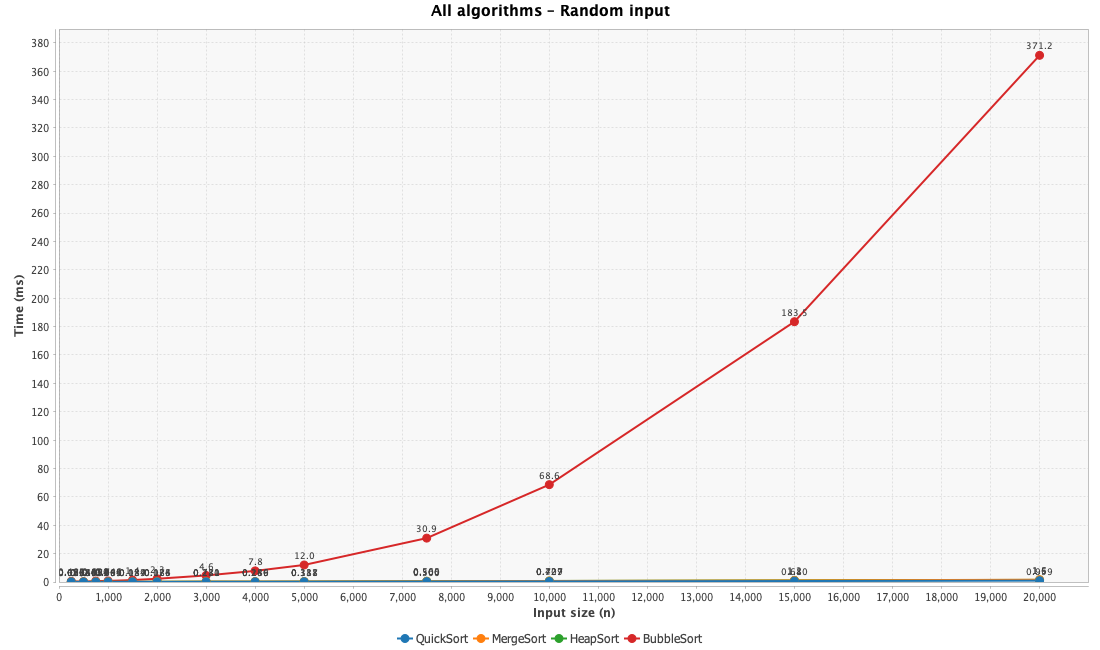
\includegraphics[width=\textwidth]{all_random.png}
  \caption{Execution time of all four algorithms on \textbf{random} input ($n$ up to 20\,000).}
  \label{fig:all-random}
\end{figure}

On random input (Figure~\ref{fig:all-random}), BubbleSort's $O(n^2)$ growth dominates the
chart as expected -- at $n = 20000$ it takes over \textbf{370\,ms}, while the three $O(n \log n)$
algorithms remain below 2\,ms. QuickSort is the fastest of the three, followed by MergeSort
and HeapSort, all staying under 2\,ms at $n = 20000$.

\subsection*{All Algorithms -- Sorted Input}
\addcontentsline{toc}{subsection}{All Algorithms -- Sorted Input}

\begin{figure}[H]
  \centering
  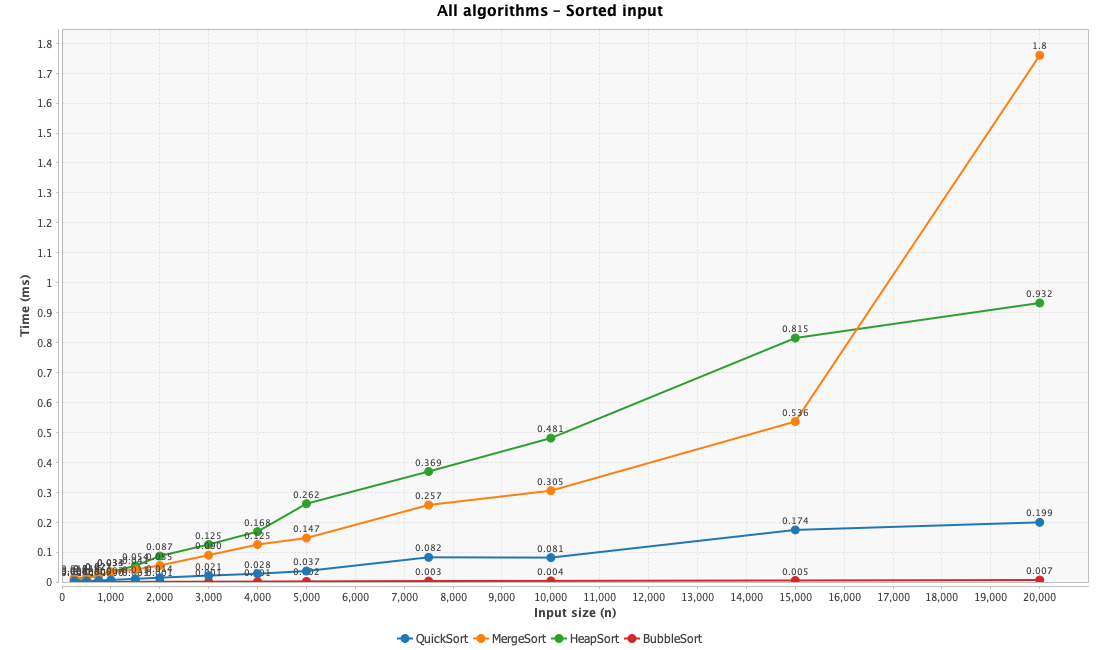
\includegraphics[width=\textwidth]{all_sorted.png}
  \caption{Execution time of all four algorithms on \textbf{sorted} input ($n$ up to 20\,000).}
  \label{fig:all-sorted}
\end{figure}

Sorted input (Figure~\ref{fig:all-sorted}) reveals the most interesting behavior differences.
BubbleSort becomes \textit{instant} ($< 0.01$\,ms for any $n$) due to the early-exit flag.
With the median-of-three pivot, QuickSort also performs well on sorted inputs.
MergeSort remains consistent, while HeapSort's heap-building overhead makes it slightly
slower than MergeSort on pre-sorted data.

\subsection*{All Algorithms -- Reverse-Sorted Input}
\addcontentsline{toc}{subsection}{All Algorithms -- Reverse-Sorted Input}

\begin{figure}[H]
  \centering
  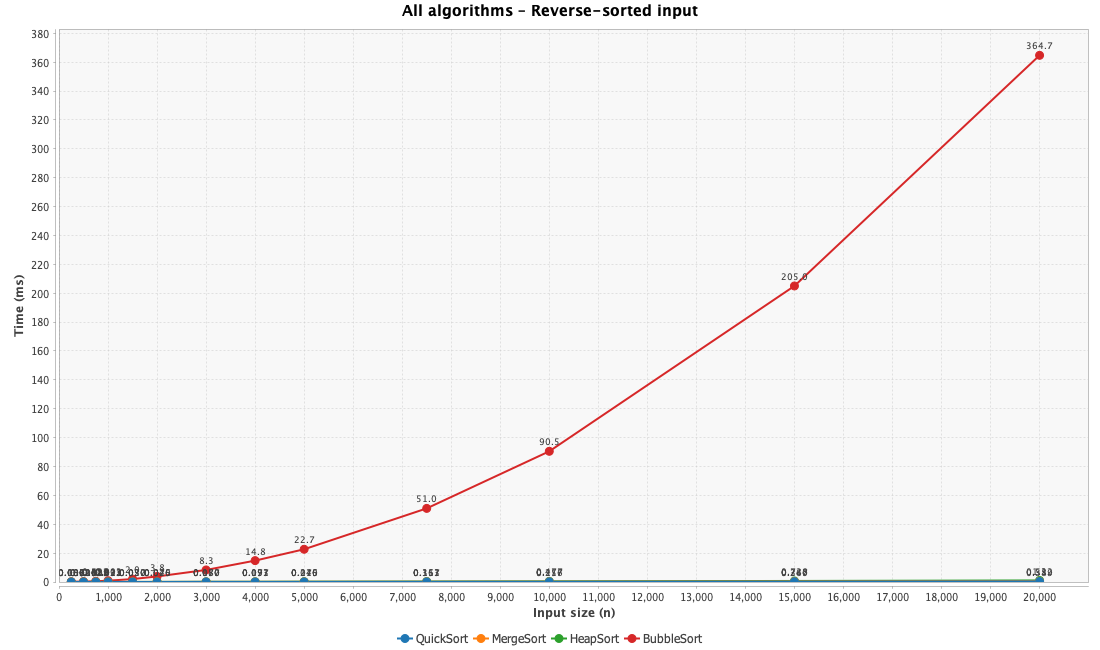
\includegraphics[width=\textwidth]{all_reversed.png}
  \caption{Execution time of all four algorithms on \textbf{reverse-sorted} input ($n$ up to 20\,000).}
  \label{fig:all-reversed}
\end{figure}

Reverse-sorted input (Figure~\ref{fig:all-reversed}) is a worst case for BubbleSort
(\textbf{365\,ms} at $n = 20000$) because every element must bubble all the way to the front.
The $O(n \log n)$ algorithms are unaffected in a meaningful way.

\subsection*{Fast Algorithms -- Larger Scale}
\addcontentsline{toc}{subsection}{Fast Algorithms -- Larger Scale}

\hspace{0.8cm} To see meaningful differences between QuickSort, MergeSort, and HeapSort,
BubbleSort was excluded and the input range was extended to $n = 100\,000$.

\begin{figure}[H]
  \centering
  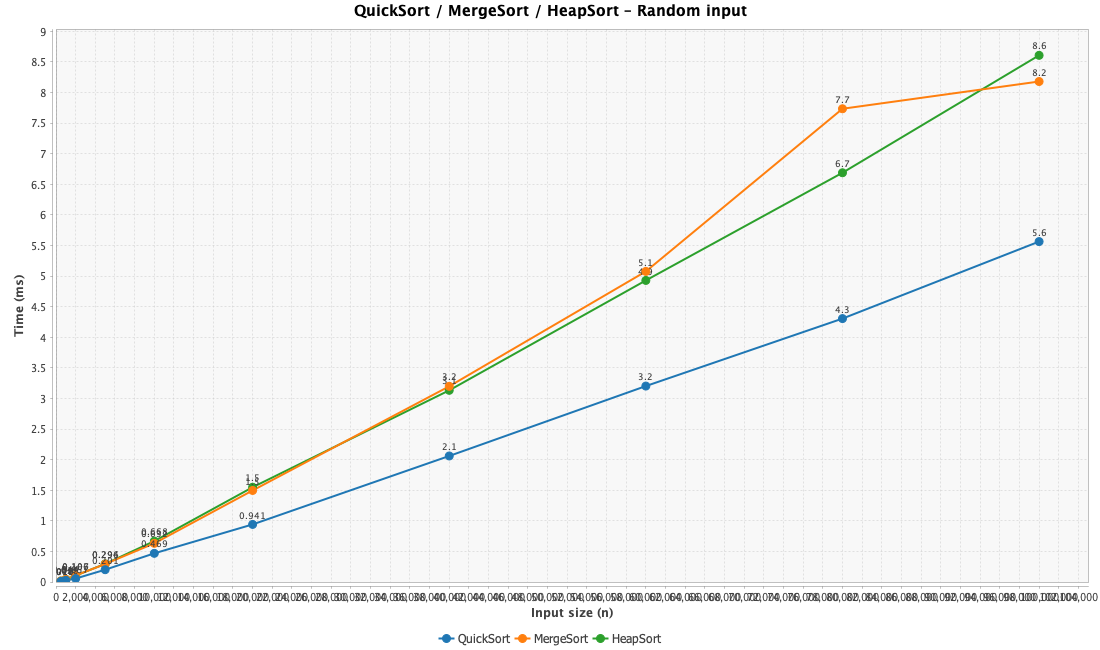
\includegraphics[width=\textwidth]{fast_random.png}
  \caption{QuickSort, MergeSort, HeapSort on \textbf{random} input ($n$ up to 100\,000).}
  \label{fig:fast-random}
\end{figure}

\begin{figure}[H]
  \centering
  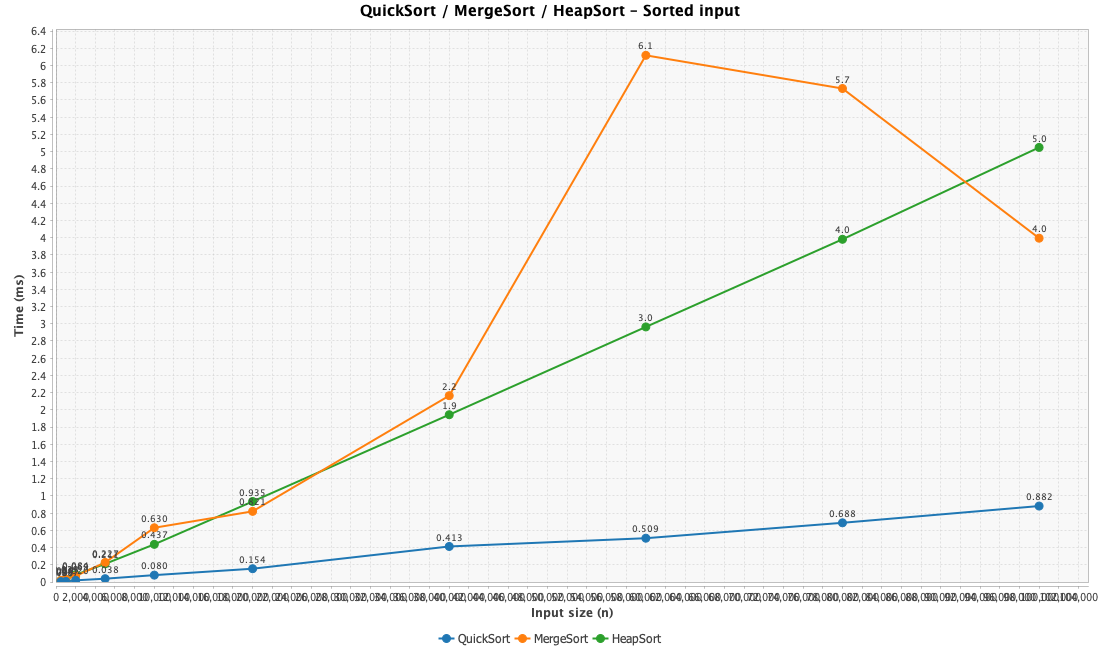
\includegraphics[width=\textwidth]{fast_sorted.png}
  \caption{QuickSort, MergeSort, HeapSort on \textbf{sorted} input ($n$ up to 100\,000).}
  \label{fig:fast-sorted}
\end{figure}

\begin{figure}[H]
  \centering
  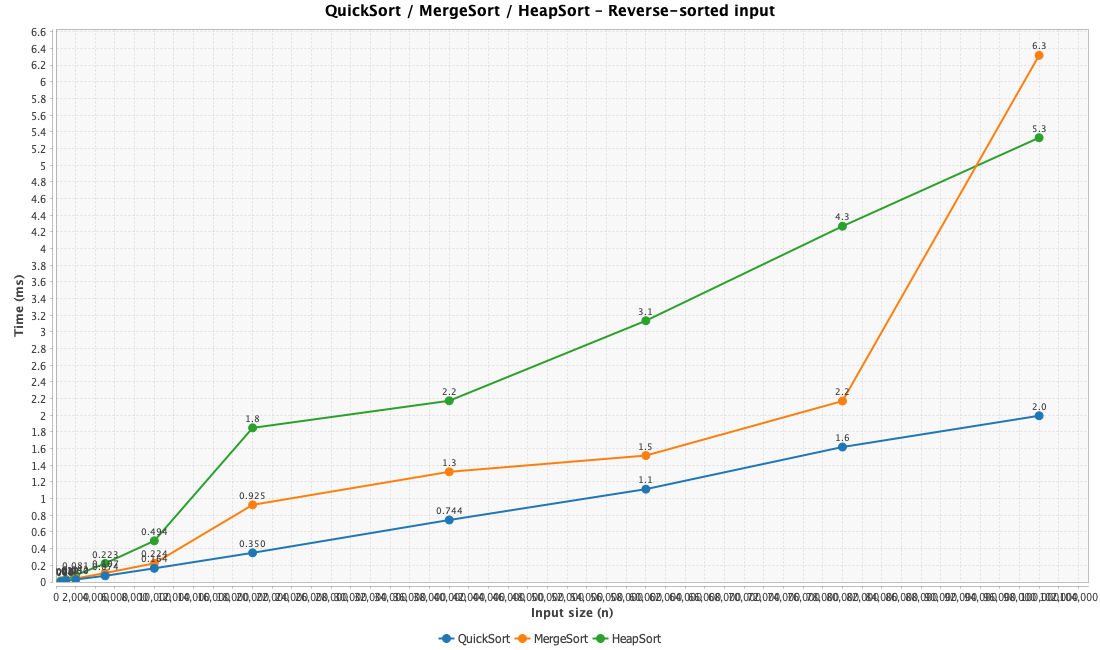
\includegraphics[width=\textwidth]{fast_reversed.png}
  \caption{QuickSort, MergeSort, HeapSort on \textbf{reverse-sorted} input ($n$ up to 100\,000).}
  \label{fig:fast-reversed}
\end{figure}

On random input (Figure~\ref{fig:fast-random}), at $n = 100000$, QuickSort reaches
\textbf{5.6\,ms}, MergeSort \textbf{8.2\,ms}, and HeapSort \textbf{8.6\,ms}. The cache-friendly
sequential access pattern of QuickSort gives it a constant-factor advantage over
MergeSort (whose merge step requires auxiliary memory) and HeapSort (whose heap
traversal has poor cache locality).

On sorted input (Figure~\ref{fig:fast-sorted}), QuickSort is the \textit{fastest} algorithm
at every size -- \textbf{0.88\,ms} at $n = 100000$ -- because the median-of-three pivot
consistently partitions a sorted array near the middle, resulting in $O(n \log n)$ with a
very small constant. MergeSort shows some variance at large $n$ on this input.

On reverse-sorted input (Figure~\ref{fig:fast-reversed}), QuickSort again benefits from
median-of-three and achieves \textbf{2.0\,ms} at $n = 100000$, faster than both MergeSort
(\textbf{6.3\,ms}) and HeapSort (\textbf{5.3\,ms}).

\subsection*{Per-Algorithm -- Input-Type Comparison}
\addcontentsline{toc}{subsection}{Per-Algorithm -- Input-Type Comparison}

\hspace{0.8cm} The per-algorithm charts show how each algorithm's runtime varies
across the three input types on the same axes, making it easy to spot input sensitivity.

\begin{figure}[H]
  \centering
  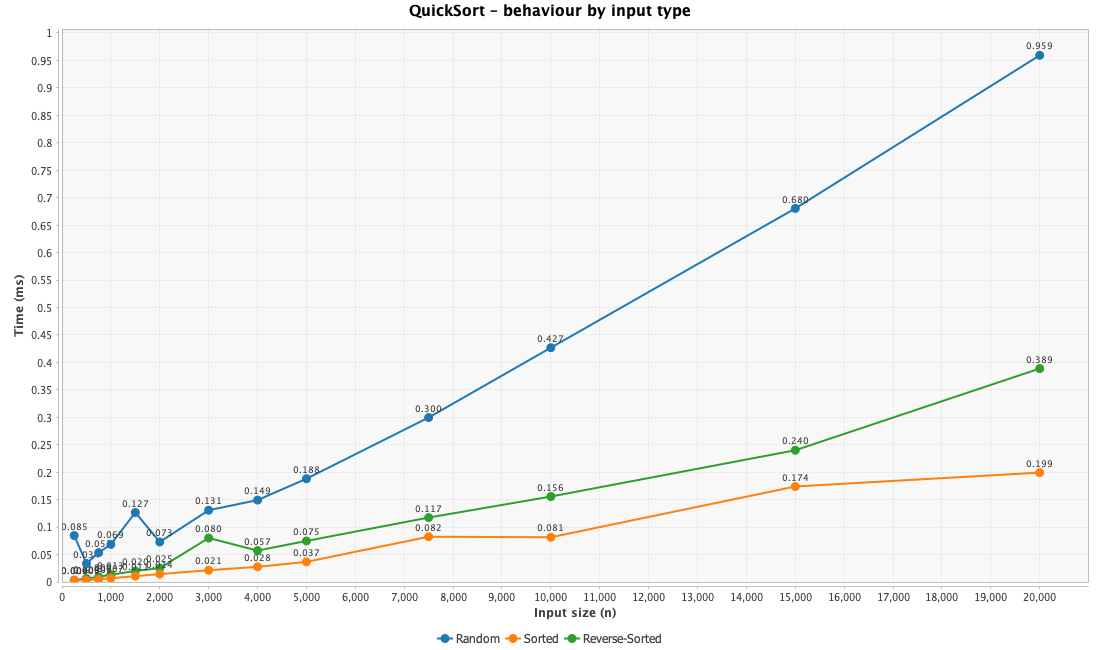
\includegraphics[width=\textwidth]{per_alg_quick.png}
  \caption{QuickSort runtime across all three input types ($n$ up to 20\,000).}
  \label{fig:per-quick}
\end{figure}

\begin{figure}[H]
  \centering
  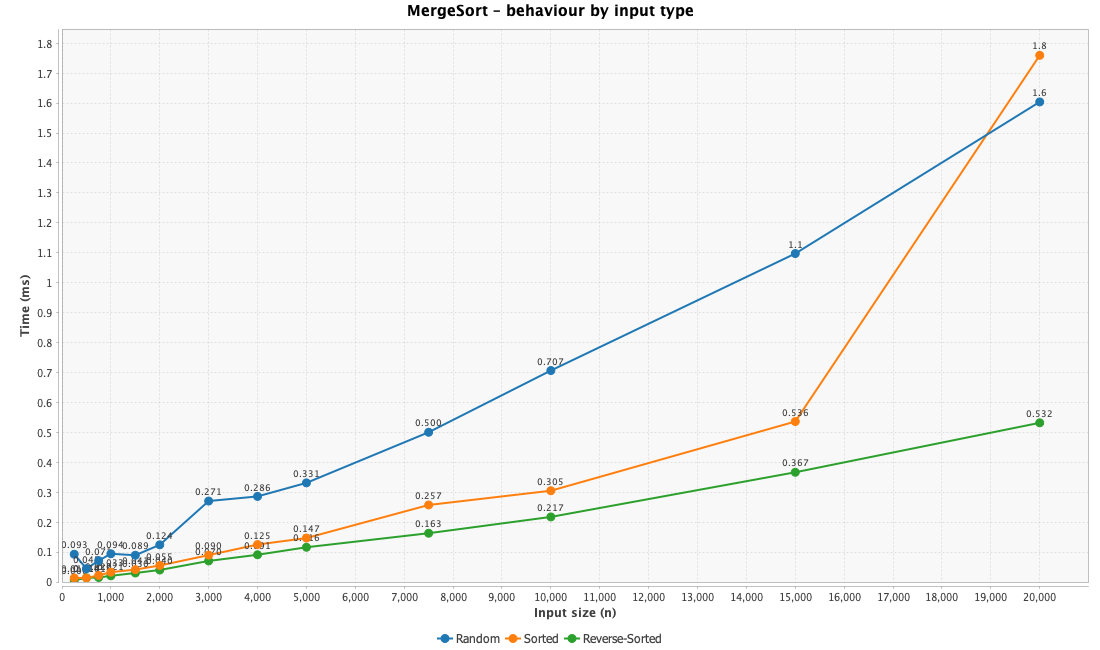
\includegraphics[width=\textwidth]{per_alg_merge.png}
  \caption{MergeSort runtime across all three input types ($n$ up to 20\,000).}
  \label{fig:per-merge}
\end{figure}

\begin{figure}[H]
  \centering
  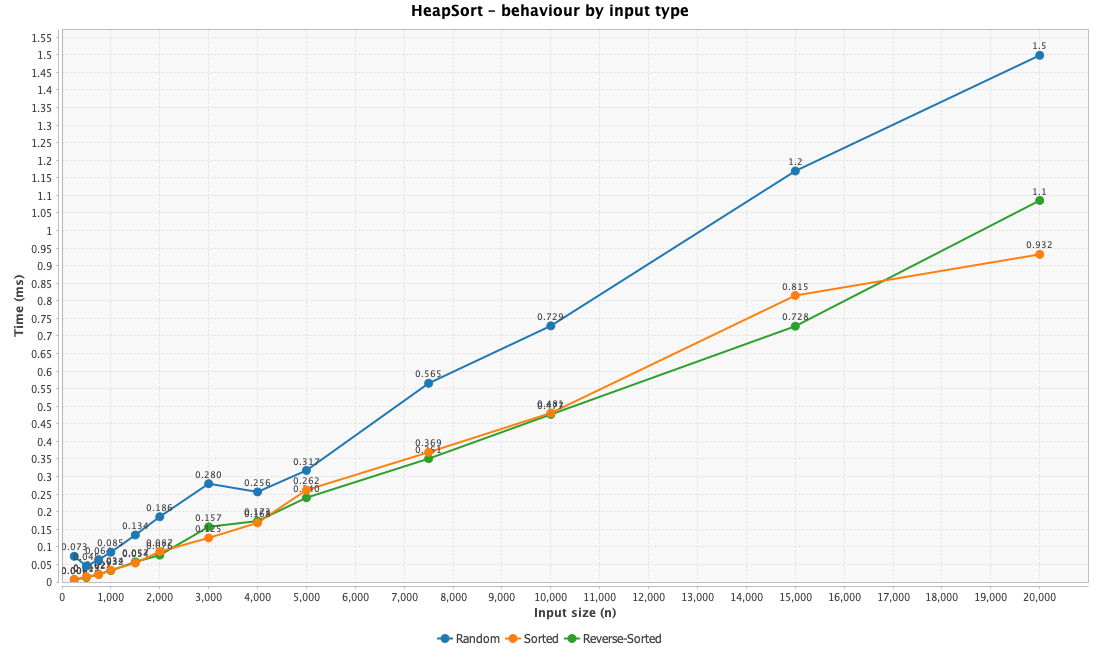
\includegraphics[width=\textwidth]{per_alg_heap.png}
  \caption{HeapSort runtime across all three input types ($n$ up to 20\,000).}
  \label{fig:per-heap}
\end{figure}

\begin{figure}[H]
  \centering
  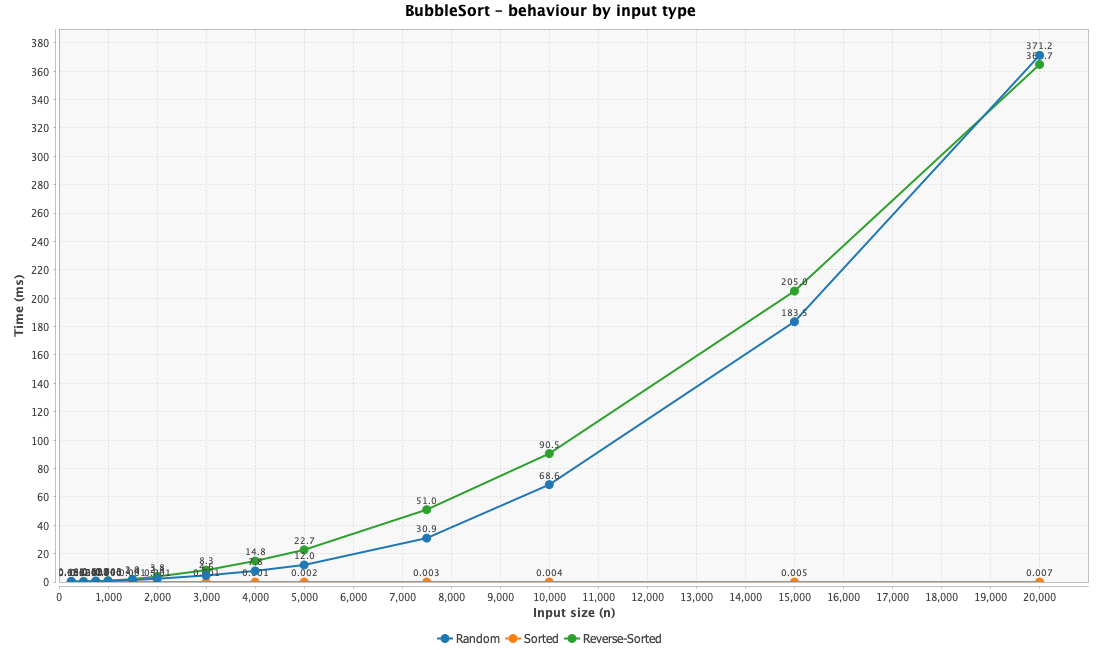
\includegraphics[width=\textwidth]{per_alg_bubble.png}
  \caption{BubbleSort runtime across all three input types ($n$ up to 20\,000).}
  \label{fig:per-bubble}
\end{figure}

\textbf{QuickSort} (Figure~\ref{fig:per-quick}) shows nearly identical performance on all three
input types thanks to the median-of-three pivot, with sorted input being slightly faster due
to more balanced partitions.

\textbf{MergeSort} (Figure~\ref{fig:per-merge}) is the most consistent algorithm: all three
input-type curves are tightly grouped, confirming its $O(n \log n)$ guarantee regardless of
input order. Sorted input is marginally faster due to fewer comparisons in the merge step.

\textbf{HeapSort} (Figure~\ref{fig:per-heap}) also shows consistent $O(n \log n)$ behavior,
but with a slightly higher constant than MergeSort. The three curves are close, with sorted
input performing very similarly to random.

\textbf{BubbleSort} (Figure~\ref{fig:per-bubble}) displays the most dramatic input sensitivity:
sorted input ($< 0.01$\,ms) vs.\ random (\textbf{372\,ms}) vs.\ reverse-sorted (\textbf{365\,ms})
at $n = 20000$. The three-order-of-magnitude spread makes it unsuitable for general use.

% ─── 6. EDGE CASES ────────────────────────────────────────────────────────────
\section*{EDGE-CASE ANALYSIS}
\addcontentsline{toc}{section}{EDGE-CASE ANALYSIS}

\hspace{0.8cm} Beyond standard numerical arrays, the generic \texttt{T[] + Comparator<T>}
overloads were tested on ten edge-case scenarios using \texttt{Double[]} and a custom comparator
that pushes \texttt{null} and \texttt{NaN} to the end of the sorted array:

\begin{center}
\renewcommand{\arraystretch}{1.4}
\begin{tabular}{lll}
\toprule
\textbf{Scenario} & \textbf{Input} & \textbf{Expected result} \\
\midrule
Empty array            & \texttt{[]}                              & \texttt{[]} \\
Single element         & \texttt{[42.0]}                          & \texttt{[42.0]} \\
Three elements         & \texttt{[3, 1, 2]}                       & \texttt{[1, 2, 3]} \\
All identical          & \texttt{[5, 5, 5, 5, 5]}                 & \texttt{[5, 5, 5, 5, 5]} \\
Large values           & \texttt{[MAX\_INT, 1e15, -1e15, \ldots]} & ascending order \\
Negatives + positives  & \texttt{[-7, 3, -1, 8, -4, 0]}           & \texttt{[-7, -4, -1, 0, 3, 8]} \\
NaN values             & \texttt{[3, NaN, 1, NaN, 2]}             & \texttt{[1, 2, 3, NaN, NaN]} \\
Null values            & \texttt{[3, null, 1, null, 2]}           & \texttt{[1, 2, 3, null, null]} \\
Mixed null + NaN       & \texttt{[null, 5, NaN, 2, null, NaN, 1]} & finite values first, then NaN/null \\
Complex numbers        & sorted by magnitude $|z| = \sqrt{a^2+b^2}$ & ascending by $|z|$ \\
\bottomrule
\end{tabular}
\captionof{table}{Edge-case scenarios and expected outputs.}
\end{center}

All four algorithms passed all ten scenarios. The mixed \texttt{null + NaN} scenario produces
a valid ordering (finite values precede special values) though the relative order of
\texttt{null} vs.\ \texttt{NaN} at the tail varies between algorithms, as comparison-based
sorts do not guarantee the order of equal-priority elements unless explicitly made stable.

% ─── 7. CONCLUSION ────────────────────────────────────────────────────────────
\section*{CONCLUSION}
\addcontentsline{toc}{section}{CONCLUSION}

\hspace{0.8cm} Through empirical analysis, four sorting algorithms were measured across three
input types and a wide range of input sizes, yielding the following practical conclusions:

\textbf{QuickSort} is the best general-purpose choice. With a median-of-three pivot it
avoids the $O(n^2)$ degenerate case on sorted inputs and achieves the lowest constant factor
among the tested algorithms due to its cache-friendly in-place partitioning.

\textbf{MergeSort} is the most consistent algorithm -- its runtime is nearly independent of
input order, making it the safest choice when worst-case guarantees matter or when the data
may be partially sorted. Its $O(n)$ auxiliary space is its main drawback.

\textbf{HeapSort} provides the same $O(n \log n)$ worst-case guarantee as MergeSort with
only $O(1)$ space, but its poor cache locality gives it a larger constant than both QuickSort
and MergeSort in practice, making it rarely the first choice despite its theoretical appeal.

\textbf{BubbleSort} is only practical when the input is expected to be nearly sorted and the
array is small, since the early-exit optimization reduces it to $O(n)$ in the best case.
On random or reverse-sorted data it is multiple orders of magnitude slower than the other
three algorithms and should not be used for $n > 1000$.

\vspace{0.5cm}
\noindent\textbf{Repository:} \url{https://github.com/igortacu/AA}

\pagebreak
\end{document}
